\documentclass{../beamer_template/myBeamer}


\DeclareMathOperator{\Cov}{Cov}
\DeclareMathOperator{\Var}{Var}
\DeclareMathOperator{\E}{\mathbb{E}}
\DeclareMathOperator{\Proba}{\mathbb{P}}

\newcommand{\Covb}[2]{\ensuremath{\Cov\!\left[#1,#2\right]}}
\newcommand{\Eb}[1]{\ensuremath{\E\!\left[#1\right]}}
\newcommand{\Pb}[1]{\ensuremath{\Proba\!\left[#1\right]}}
\newcommand{\Varb}[1]{\ensuremath{\Var\!\left[#1\right]}}

% norm
%\newcommand{\norm}[1]{\| #1 \|}

\newcommand{\indep}{\rotatebox[origin=c]{90}{$\models$}}





\usepackage{mathptmx,amsmath,amssymb,graphicx,bibentry,bbm,babel,ragged2e}

\makeatletter


\renewcommand{\addlogo}{
	\hfill	
	
\includegraphics[height=.4cm]{../beamer_template/figures/logos/iconOM.png}
	
\includegraphics[scale=1]{../beamer_template/figures/logos/openmole_dark.png}
}


\newcommand{\noun}[1]{\textsc{#1}}
\newcommand{\jitem}[1]{\item \begin{justify} #1 \end{justify} \vfill{}}
%\newcommand{\sframe}[2]{\frame{\frametitle{#1}\addlogo #2}}

\newenvironment{centercolumns}{\begin{columns}[c]}{\end{columns}}
%\newenvironment{jitem}{\begin{justify}\begin{itemize}}{\end{itemize}\end{justify}}

%\usetheme{Warsaw}
%\setbeamertemplate{footline}[text line]{}
%\setbeamersize{text margin left=15pt,text margin right=15pt}
%\setbeamertemplate{headline}{}
%\setbeamertemplate{footline}[frame number]
%\setbeamertemplate{navigation symbols}{}

\usetheme{Darmstadt}
\setbeamertemplate{headline}{}
\setbeamertemplate{navigation symbols}{}
\setbeamercolor{palette quaternary}{fg=primaryDarkOM, bg=primaryGreenOM}


%\setbeamercovered{transparent}
%\setbeamercolor{structure}{fg=purple!50!blue, bg=purple!50!blue}

\@ifundefined{showcaptionsetup}{}{%
 \PassOptionsToPackage{caption=false}{subfig}}
\usepackage{subfig}

\usepackage[utf8]{inputenc}
%\usepackage[T1]{fontenc}


\usepackage{tikz}

\usepackage{multirow}

\usepackage{mdframed}

%\usepackage[usenames,dvipsnames]{pstricks}
%\usepackage{auto-pst-pdf}


%\usepackage[dvipsnames]{xcolor}

\usepackage{threeparttable}


\usepackage{listings}
\lstset{language=Java} 

\makeatother



\usepackage{pifont}
%\newcommand{\cmark}{\textcolor{green}\ding{51}}
%\newcommand{\xmark}{\textcolor{red}\ding{55}}
\newcommand{\cmark}{\ding{51}}
\newcommand{\xmark}{\ding{55}}

\title[DOE/Sensitivity Analysis]{Design of Experiments and Sensitivity analysis}
\subtitle{Course and practical application}
%\author[Short Author]{Author}
\author{eX Modelo Summer School}
\date{August 31st, 2020}
\institute{
\includegraphics[scale=2]{../beamer_template/figures/logos/openmole.png}}

\begin{document}



\begin{frame}[plain]
	\titlepage
\end{frame}
\addtocounter{framenumber}{-1}

\AtBeginSection[]
{
	\frame{
		\tableofcontents[currentsection, hideallsubsections]
	}
	\addtocounter{framenumber}{-1}
}





%orthographe: eX Modelo
%S1 : les remarques sont très bien 
%Le vert ressort mal pour les titre, on voit mal


%S4: qualification du OAT : ++

%Est-ce qu'il ne faudrait pas faire un petit schéma pour expliquer chaque méthode ?

%Compliqué la partie OFAT pour commencer ... non ?
%J'ai pas compris les graphes [name = Paul] => plus expliciter et details. dire que plus de calcul.
%dixit Juste: il faut que j'essaye de virer les jugements disciplinaires
%dixit Paul : oui 

%S7: ajouter les plots sobol et grid sur le modèle zombie

%S8 : la formule est raide à cause des symboles un peu rares : le 1 à double barre, la fonction / produit $\Pi$ etc.. $\implies$ garder l'intuition de la discrepancy comme la faculté de "bien couvrir" l'espace

%Que signifie l'«intégrale» qui sert d'évaluation des séquences de nombres (1/N, 1/ $\sqrt N$ , etc..)

%S11 : cool , explicite et illustratif


%/!\ Intercaler la manip avant de passer à morris/saltelli /!\

%manip : grid ; sobol

%ajouter elements de texte explication formule discrepance

%manip : saltelli - NO : morris

%ajouter slides : tableau de synthese avantage / probleme of each method (after sampling and after sensitivity)

%aller plus lentement - chaque methode clair - segmenter.


%\section{Introduction}


\sframe{Design of Experiments}{
\justify

\begin{itemize}
	\item Interactive model exploration by hand and the need for preliminary experiments
    \item The Design of Experiments (DOE) as the definition of computational experiments to extract information from the simulation model
    \item Example: NetLogo behavior space: basic grid DOE
    \item Sensitivity analysis as an advanced DOE
\end{itemize}

\bigskip

\textbf{Remark 1:} \textit{terminology strongly depends on disciplines and practices}

\medskip

\textbf{Remark 2:} \textit{most are generally \textbf{preliminary experiments} to prepare more elaborated, question-related, experiments}


}



\sframe{Outline}{
\tableofcontents
}


\section{Basic experiments}


\sframe{Basic experiments}{

\justify

\textit{Provide explicitly sampling points on which the model (or its replication task) will be run: notion of \textbf{direct sampling} in OpenMOLE (corresponds to DOE in the literature)}

\bigskip

\begin{itemize}
	\item full samplings
    \item elaborated sampling for high dimensions given a low computational budget (\textbf{the curse of dimensionality})
\end{itemize}

}

\sframe{OpenMOLE syntax}{

\textbf{Syntax of the direct sampling method in OpenMOLE:}

\medskip

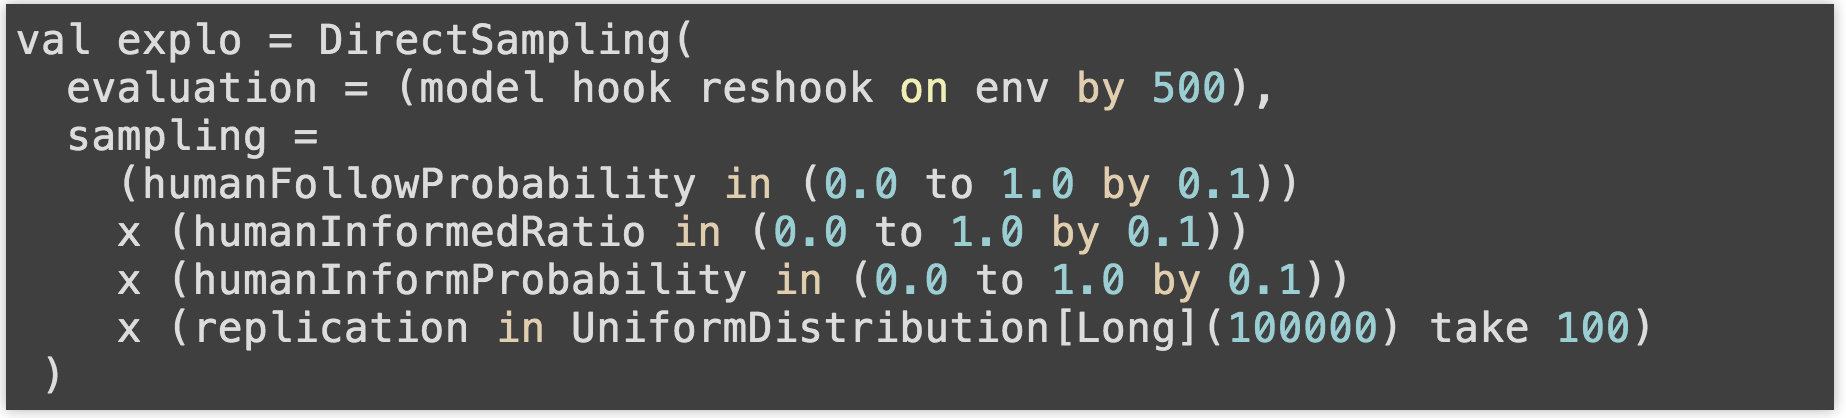
\includegraphics[width=\textwidth]{figures/directSamplingcode.png}

%\texttt{
%val explo = DirectSampling(\\
% \hspace{1cm}evaluation = model,\\
% \hspace{1cm}sampling = \dots \\
%)
%}
}


\sframe{One factor at a time}{
  
  
\justify  
  
Cheapest and intuitive DOE: \textit{all factors have nominal values and a discrete variation set, in which each is varied while others remaining fixed}

\bigskip

\begin{itemize}
  \item when model is slow - or computational budget highly limited
  \item does not capture interaction between parameters, and highly dependent on nominal values
  \item seen as a bad practice \textbf{BUT} useful for models taking significant time, and prone to thematic interpretation
\end{itemize}

  
}

\sframe{Example where One-At-a-Time fails}{

 %<img width=600 src=https://miniocodimd.openmole.org:443/codimd/uploads/upload_82c20b2e74a3f5b96a0fc227311cd516.png/>
 
 \begin{center}
 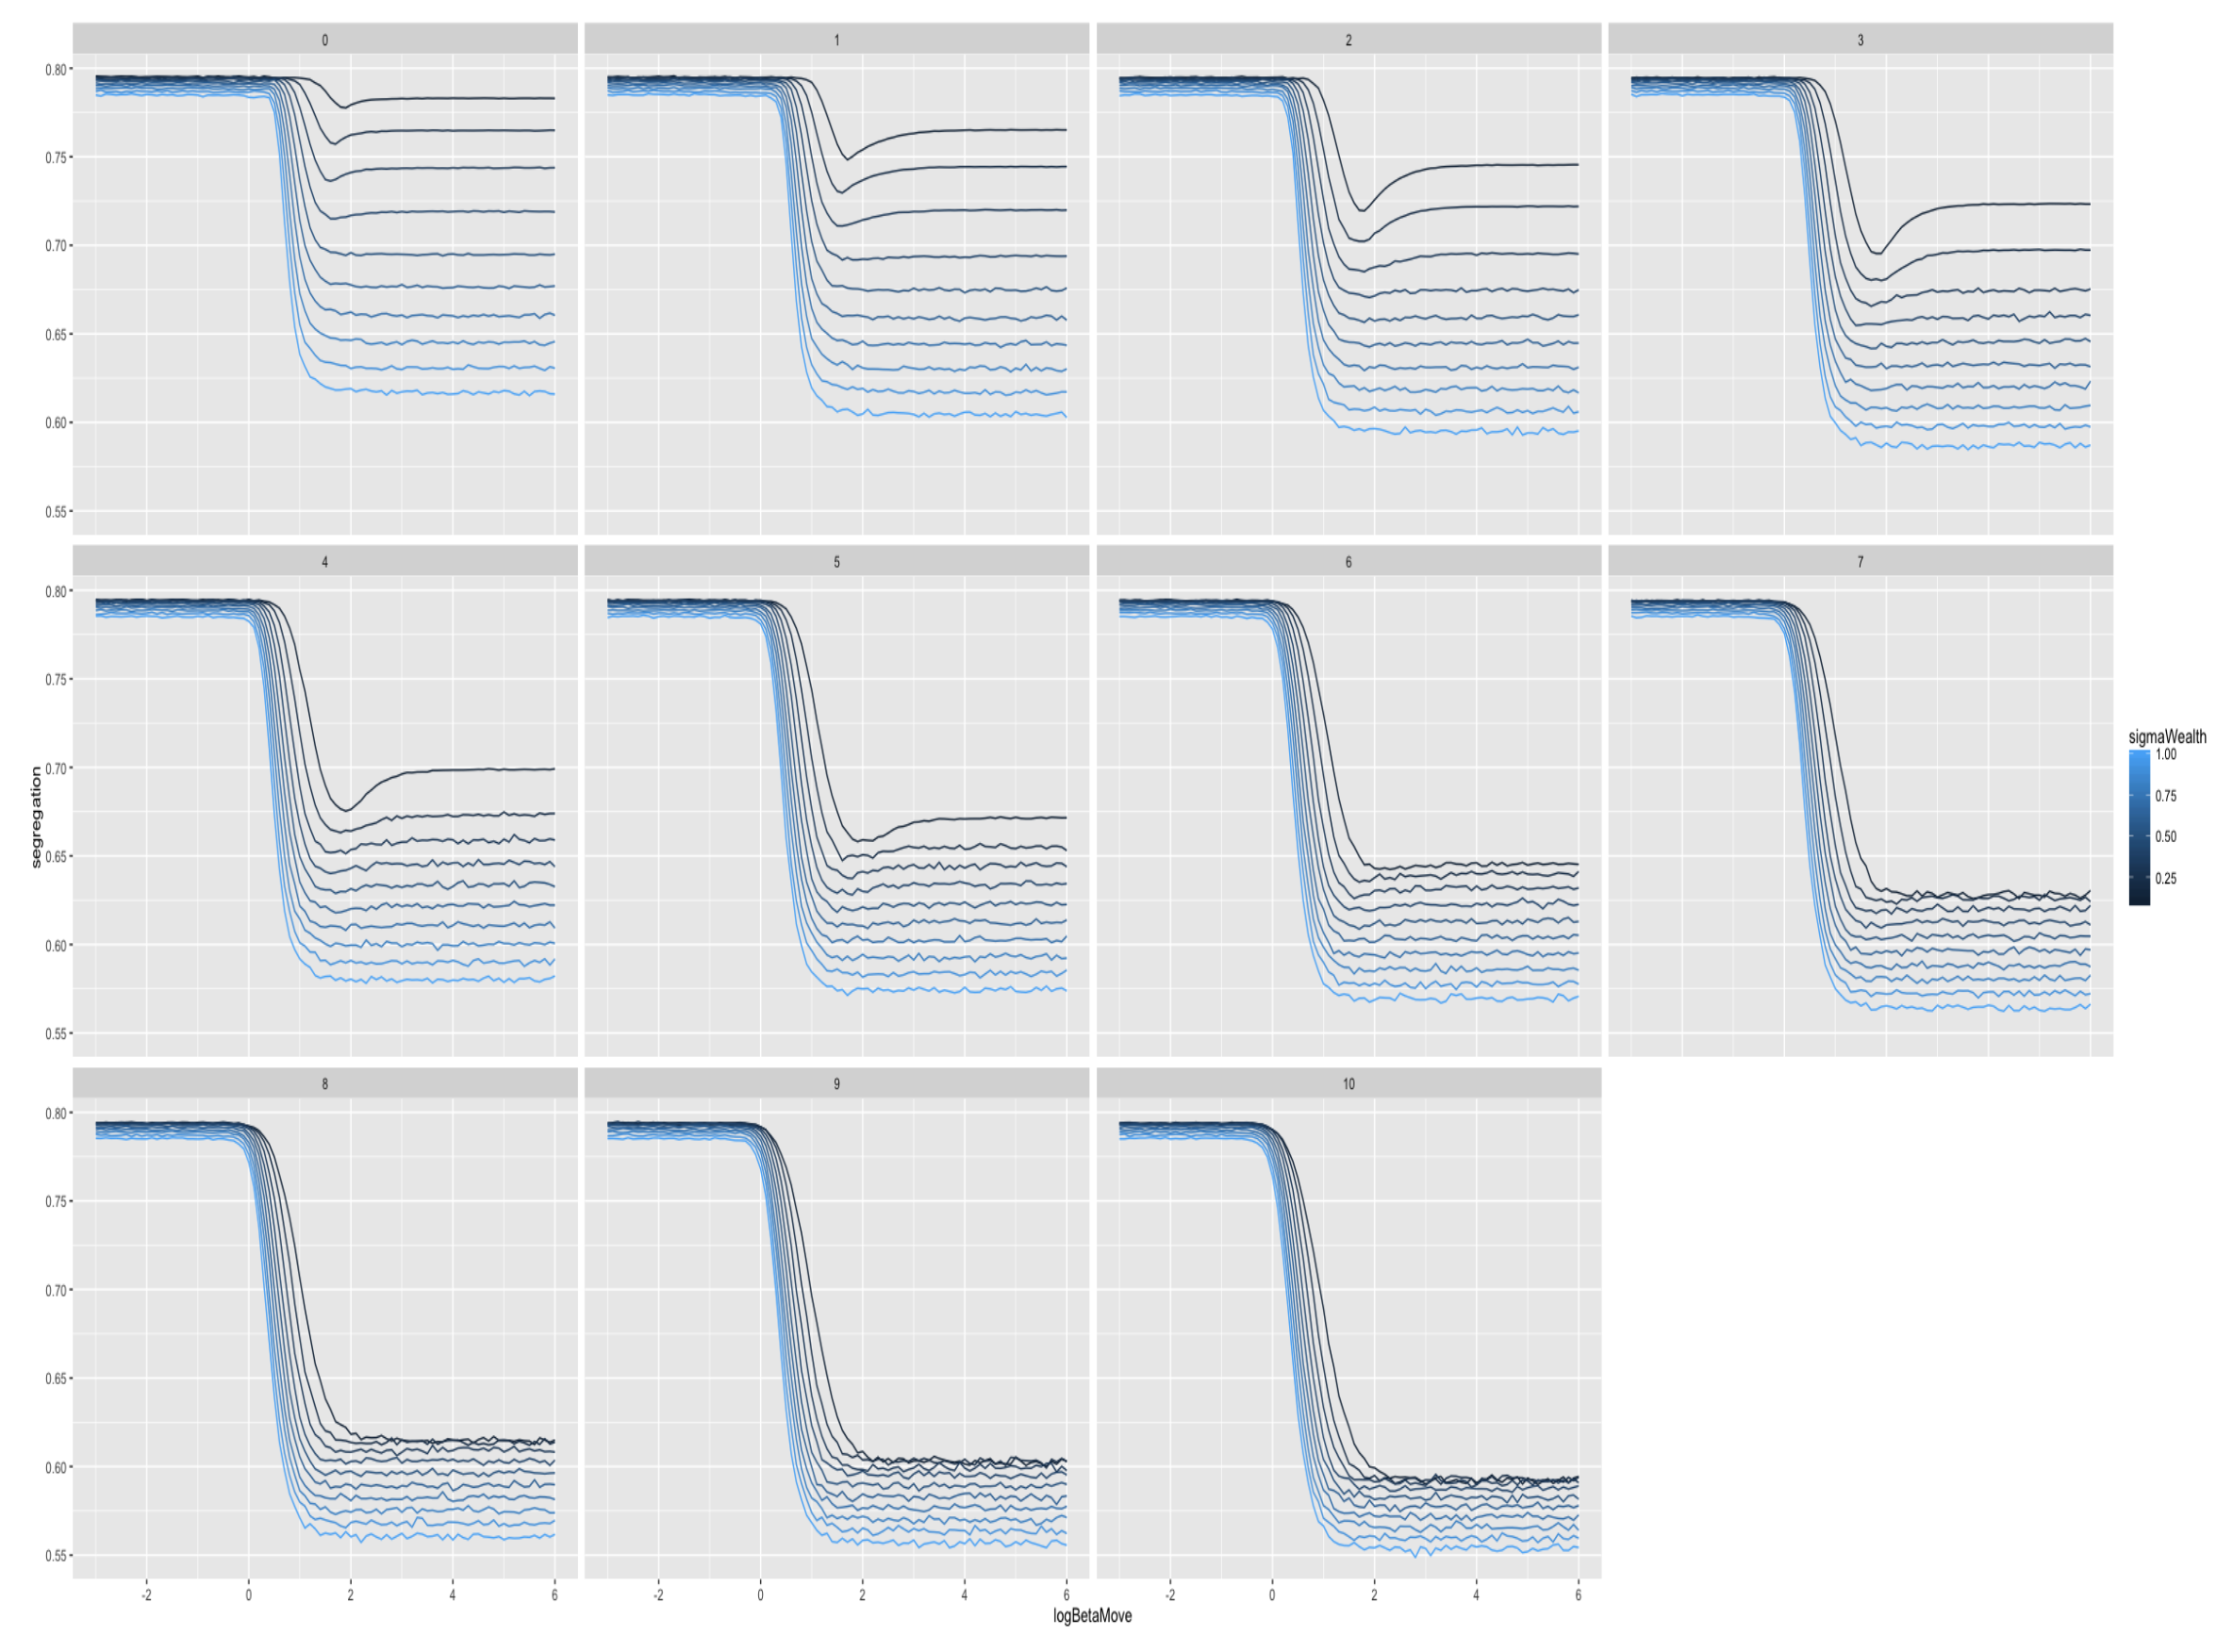
\includegraphics[width=0.8\textwidth]{figures/example_oatfailure.png}
 \end{center}
 
 \footnotesize
 
 \textit{Indicator variations in a 3D parameter space: some nominal values make non-monotonous effects disappear}
 

}


\sframe{Grid sampling}{



Brute force DOE: \textit{ensemble product of discrete variation ranges for factors (usually a regular grid but not necessarily)}

\bigskip


\begin{itemize}
  \item quickly limited by the curse of dimensionality - in practice still powerful with a quick model and a low number of parameters
  \item naive approach, but remains only DOE for many "simulation-newcomers" disciplines
\end{itemize}


}


\sframe{Syntax of samplings}{

  \textbf{One-factor sampling: }

\medskip

\texttt{
 sampling = OneFactorSampling(\\
  \hspace{1cm}(x1 in (0.0 to 1.0 by 0.2)) nominal 0.5,\\
  \hspace{1cm}(x2 in (0.0 to 1.0 by 0.2)) nominal 0.5\\
 )
}

\bigskip

\textbf{Grid sampling: }


\medskip

\texttt{
sampling = \\
 \hspace{1cm} (x1 in (0.0 to 1.0 by 0.5)) x\\
 \hspace{1cm} (x2 in (0.0 to 1.0 by 0.5))
}

}


\sframe{Practical application}{



\begin{itemize}
	\item Given the described zombie model, what first experiment beyond stochasticity would be relevant ?
    \item Explore and test the \texttt{directsampling.oms} script available in the downloaded archive (see chat for link)
    %\url{} % tp download url - in chat ?
    %\item Explore results (using e.g. the OpenMOLE GUI plots)
\end{itemize}

%\textit{Resources:}
% - one script running directsampling
% - example of grid explo results
% - example of Saltelli

}

\sframe{Example of direct sampling results}{

\textit{Regular grid sampling for the three parameters of the basic ZOMBIE model, with 100 replications}

\medskip

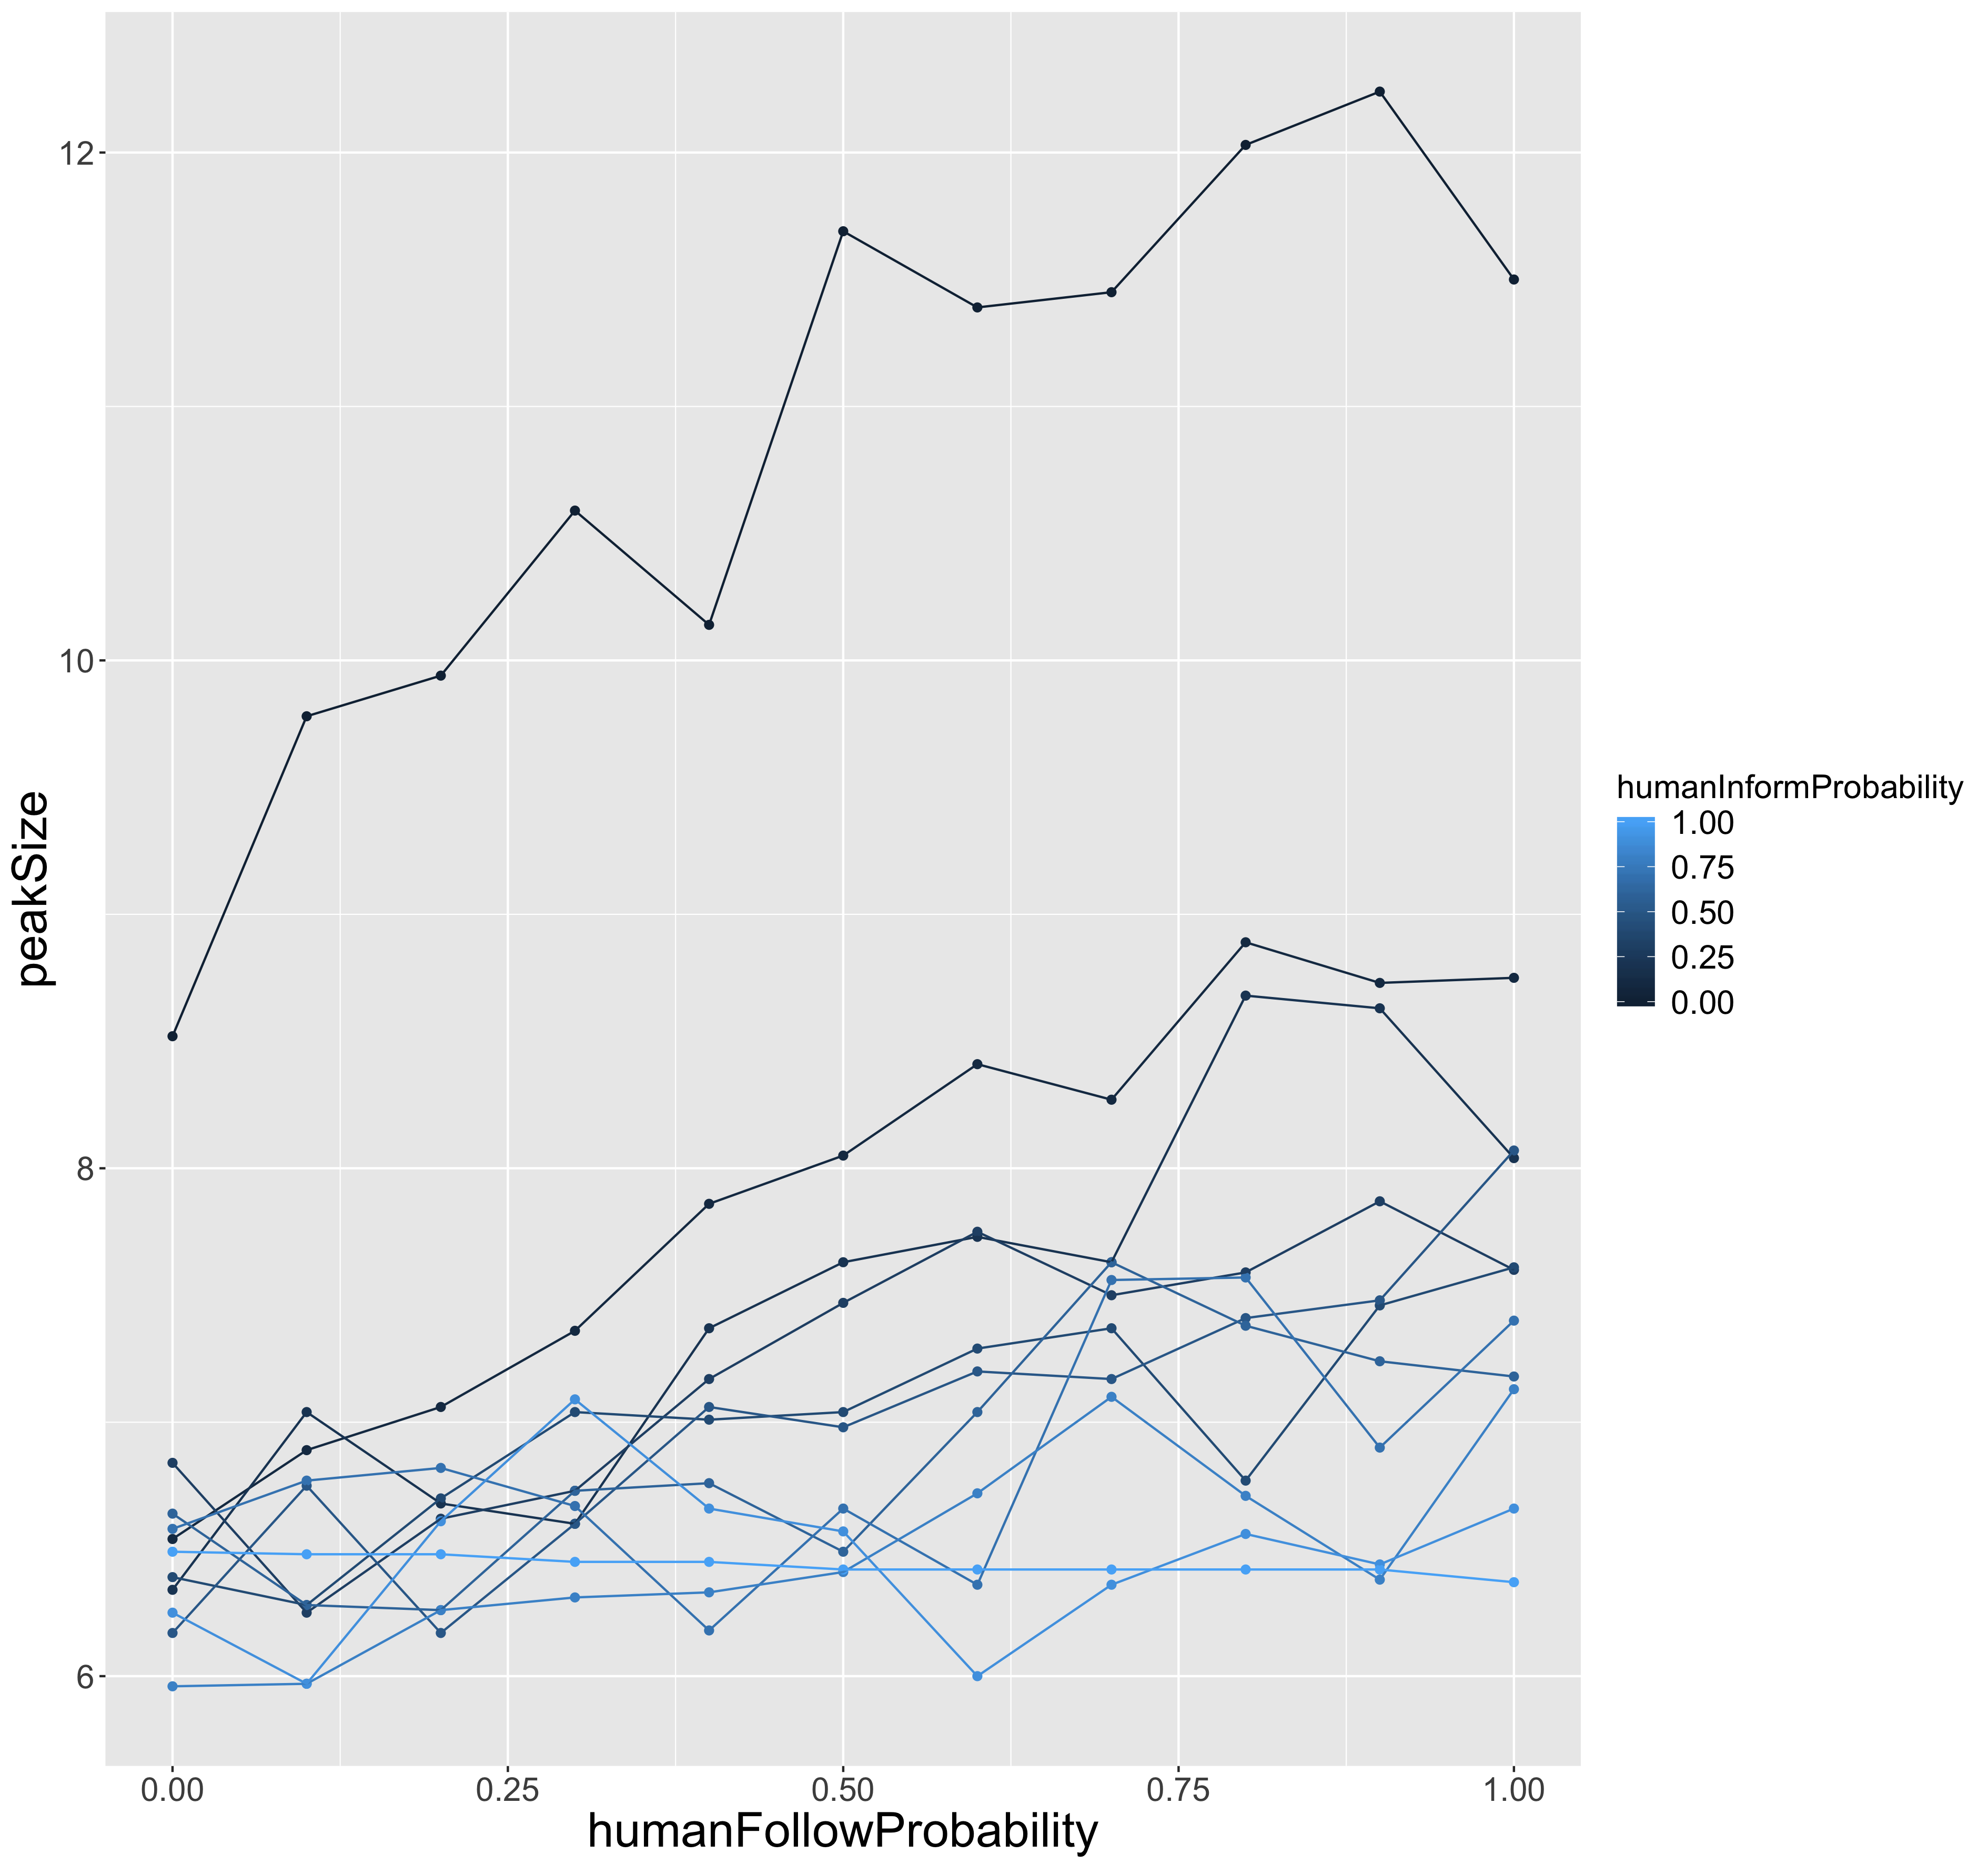
\includegraphics[width=0.48\textwidth]{figures/peakSizeAverage_p3Fixed04_humanFollowProbability_colorhumanInformProbability_facethumanInformedRatio.png}
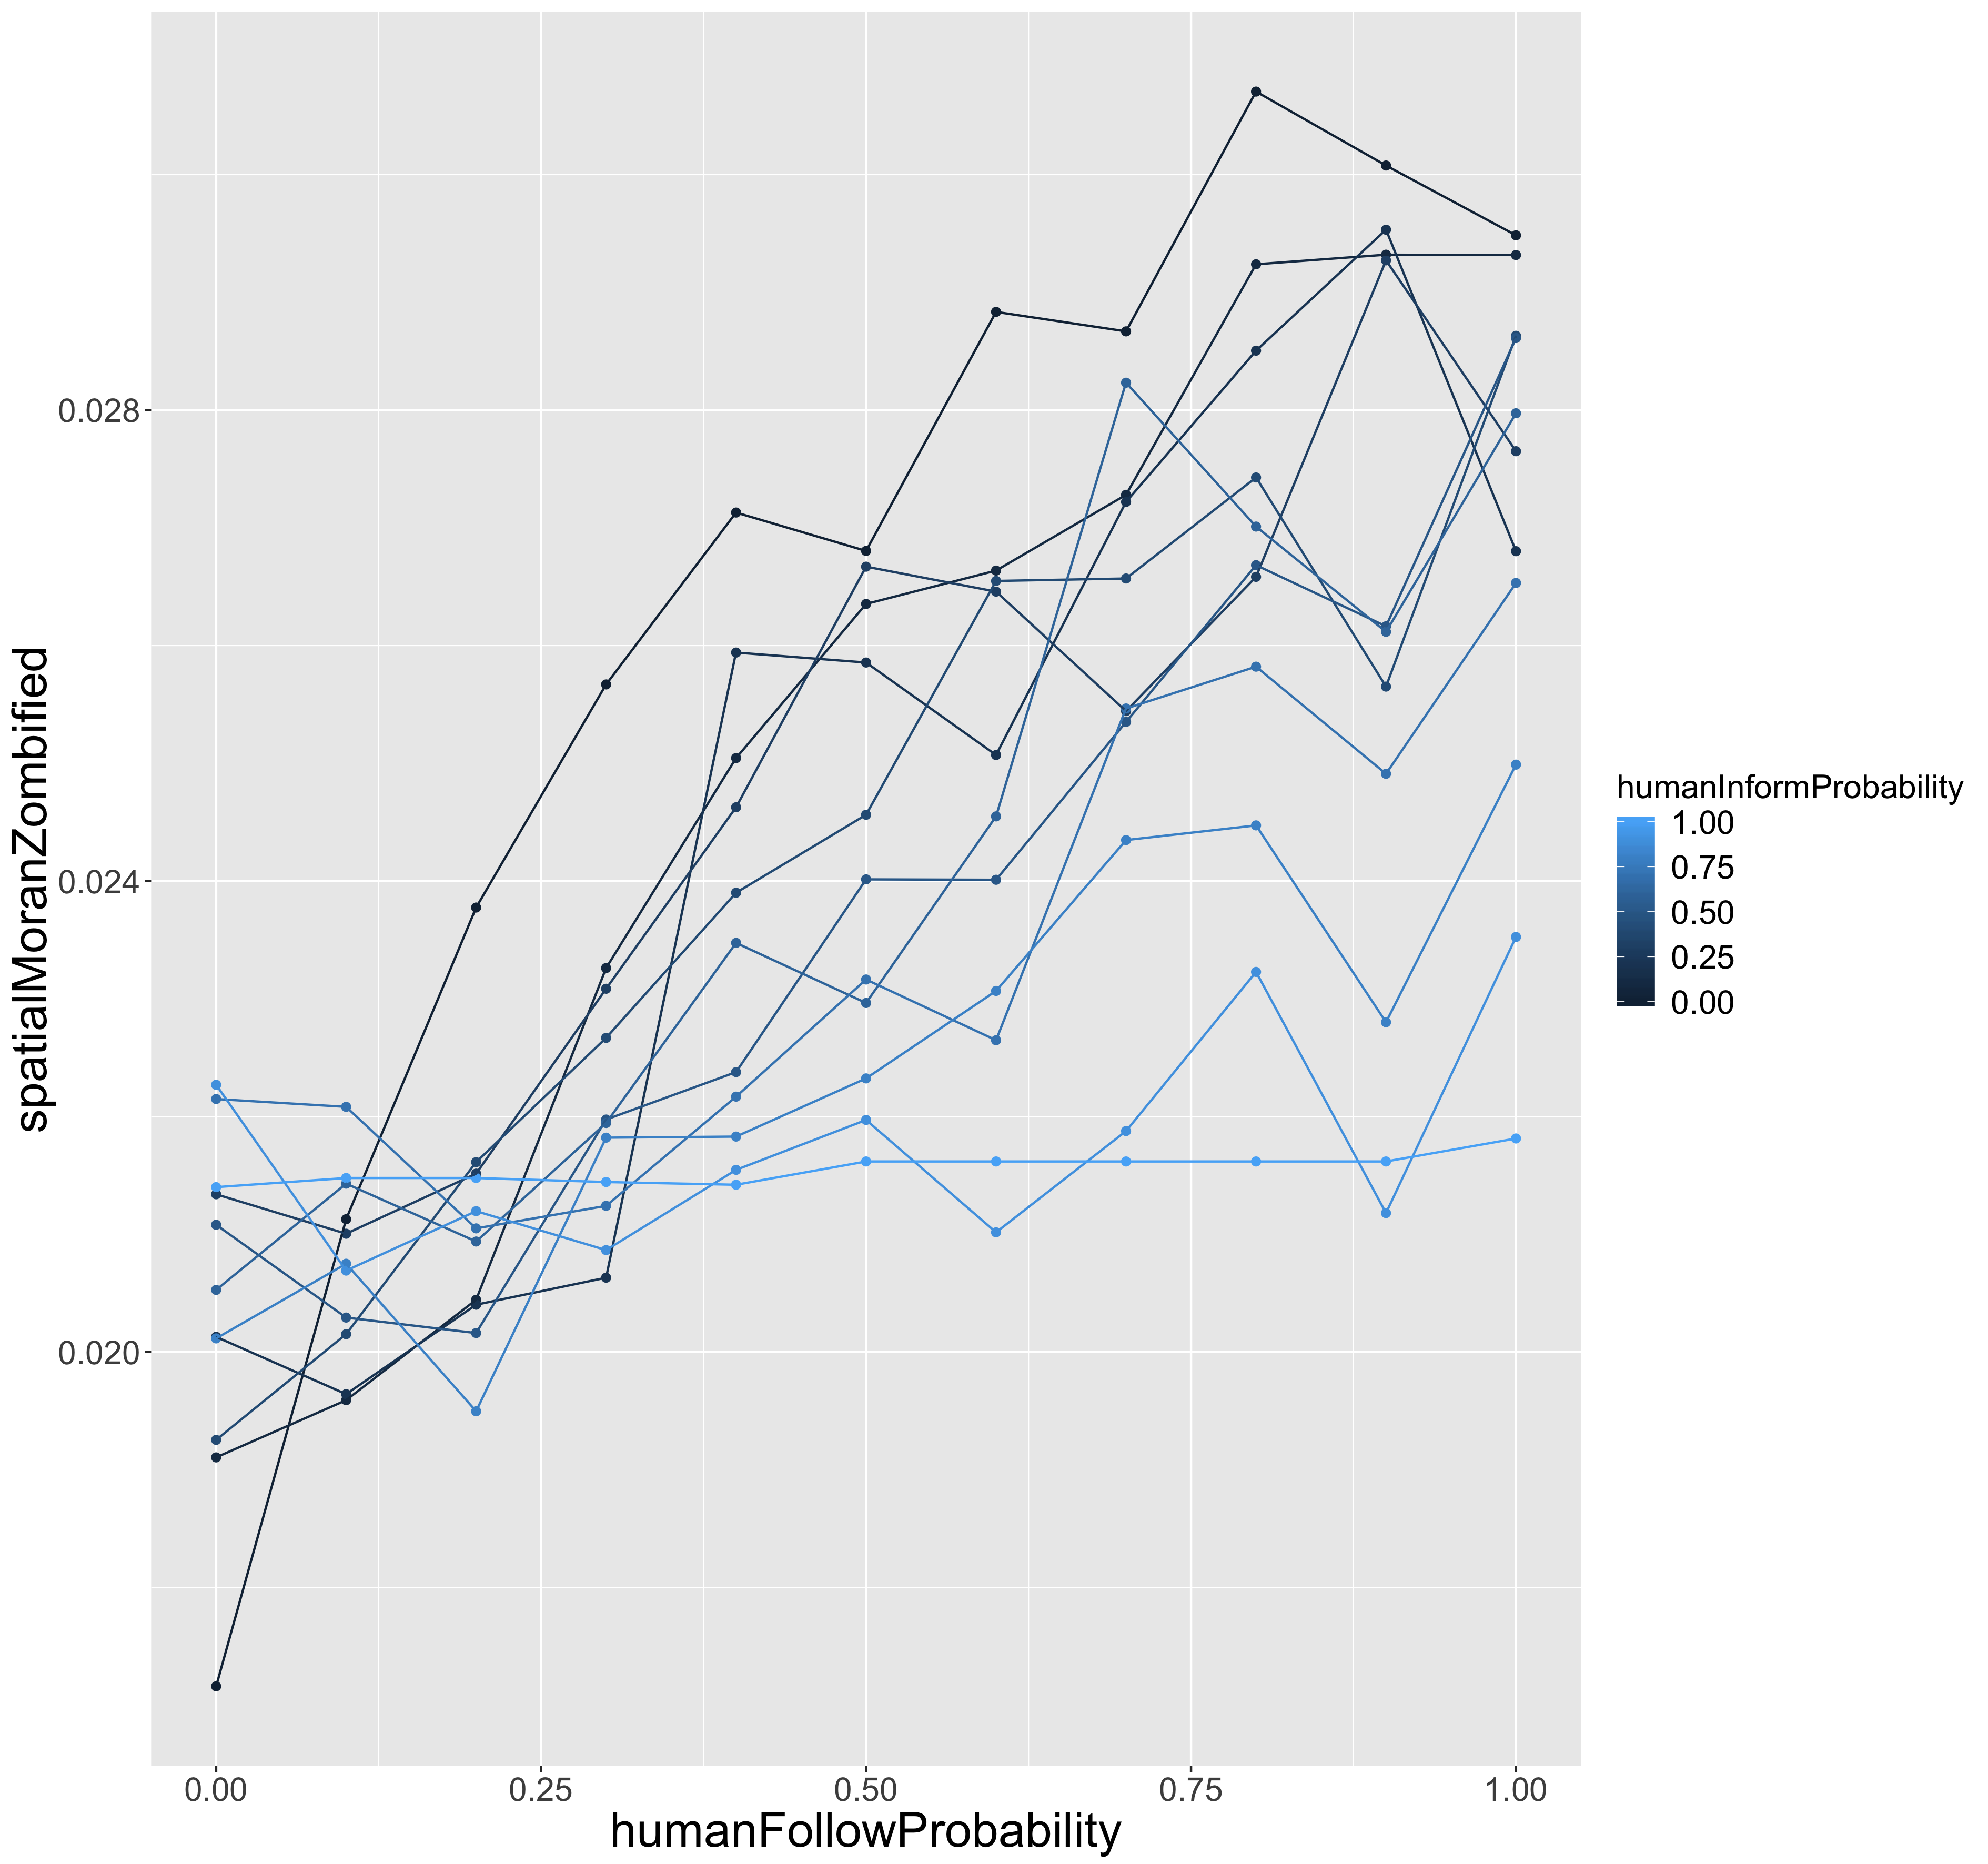
\includegraphics[width=0.48\textwidth]{figures/spatialMoranZombifiedAverage_p3Fixed04_humanFollowProbability_colorhumanInformProbability_facethumanInformedRatio.png}

}




\section{High-dimensional samplings}


\sframe{High-dimensional samplings}{

\justify

\textit{Computational limitations} $\implies$ \textit{need specific methods to efficiently sample the parameter space}

\bigskip

Different methods for improving sampling in numerical experiments given limited computational resources have been proposed, as for example:

\medskip

\begin{itemize}
	\item Sobol sequences (quicker convergence of for Monte Carlo estimation of integrals)
	\item Latin Hypercube Sampling
	\item Orthogonal sampling
\end{itemize}


}


\sframe{Low discrepancy samplings}{

\textit{Minimizing discrepancy for a point cloud: intuitively being spread evenly across the definition space}

\bigskip

%(def of discrepancy)
% The discrepancy is defined as the $L2$-norm of local discrepancy which is for normalized data points $\mathbf{X}=(x_{ij})\in \left[0,1\right]^d$, a function of $\mathbf{t}\in \left[0,1\right]^d$ comparing the number of points falling in the corresponding hypercube with its volume, by $disc(\mathbf{t}) = \frac{1}{n}\sum_i \mathbbm{1}_{\prod_j x_{ij}<t_j} - \prod_j t_j$. It is a measure of how the point cloud covers the space.

L2-discrepancy given for normalized data points $\mathbf{X}=(x_{ij})\in \left[0,1\right]^d$ by



\bigskip
\bigskip

\footnotesize

\textit{Explanation: $\prod_j t_j$ is the volume of the hypercube between $\mathbf{t}$ and the origin; the sum of indicator functions counts the points within that hypercube; the difference between expected volume and point number is integrated over the whole hypercube.}


\footnotesize

\[
\left\lVert \mathbf{t} = (t_j) \in \left[0,1\right]^d \mapsto \frac{1}{n}\sum_i \mathbbm{1}_{\prod_j x_{ij}<t_j} - \prod_j t_j \right\rVert_2
\]

}


\sframe{Latin Hypercube Sampling}{


%|x|||||
%|:--:|:--:|:--:|:--:|:--:|
%||x||||
%|||||x|
%||||x||
%|||x|||

\begin{center}
\begin{tabular}{|c|c|c|c|c|}
\hline
	x & & & & \\\hline
	 & x & & & \\\hline
	 & & & & x \\\hline
	 & & & x & \\\hline
	 & & x & & \\\hline
\end{tabular}
\end{center}

\bigskip

\textit{Latin cube: one point in each row and column; hypercube generalization in any dimension}

}



\sframe{Sobol sequence}{

\textit{Sobol sequences are a case of quasi-random sequences with low discrepancy (also Halton sequences e.g.)}

\bigskip


\begin{itemize}
	\item Estimate integrals in $1/N$ instead of $1/\sqrt{N}$ with random sampling
	\item Constructed recursively (using bit representations)
\end{itemize}

}

\sframe{Comparison of samplings}{

For $N=2500$ samples in 2 dimensions

\centering

\medskip

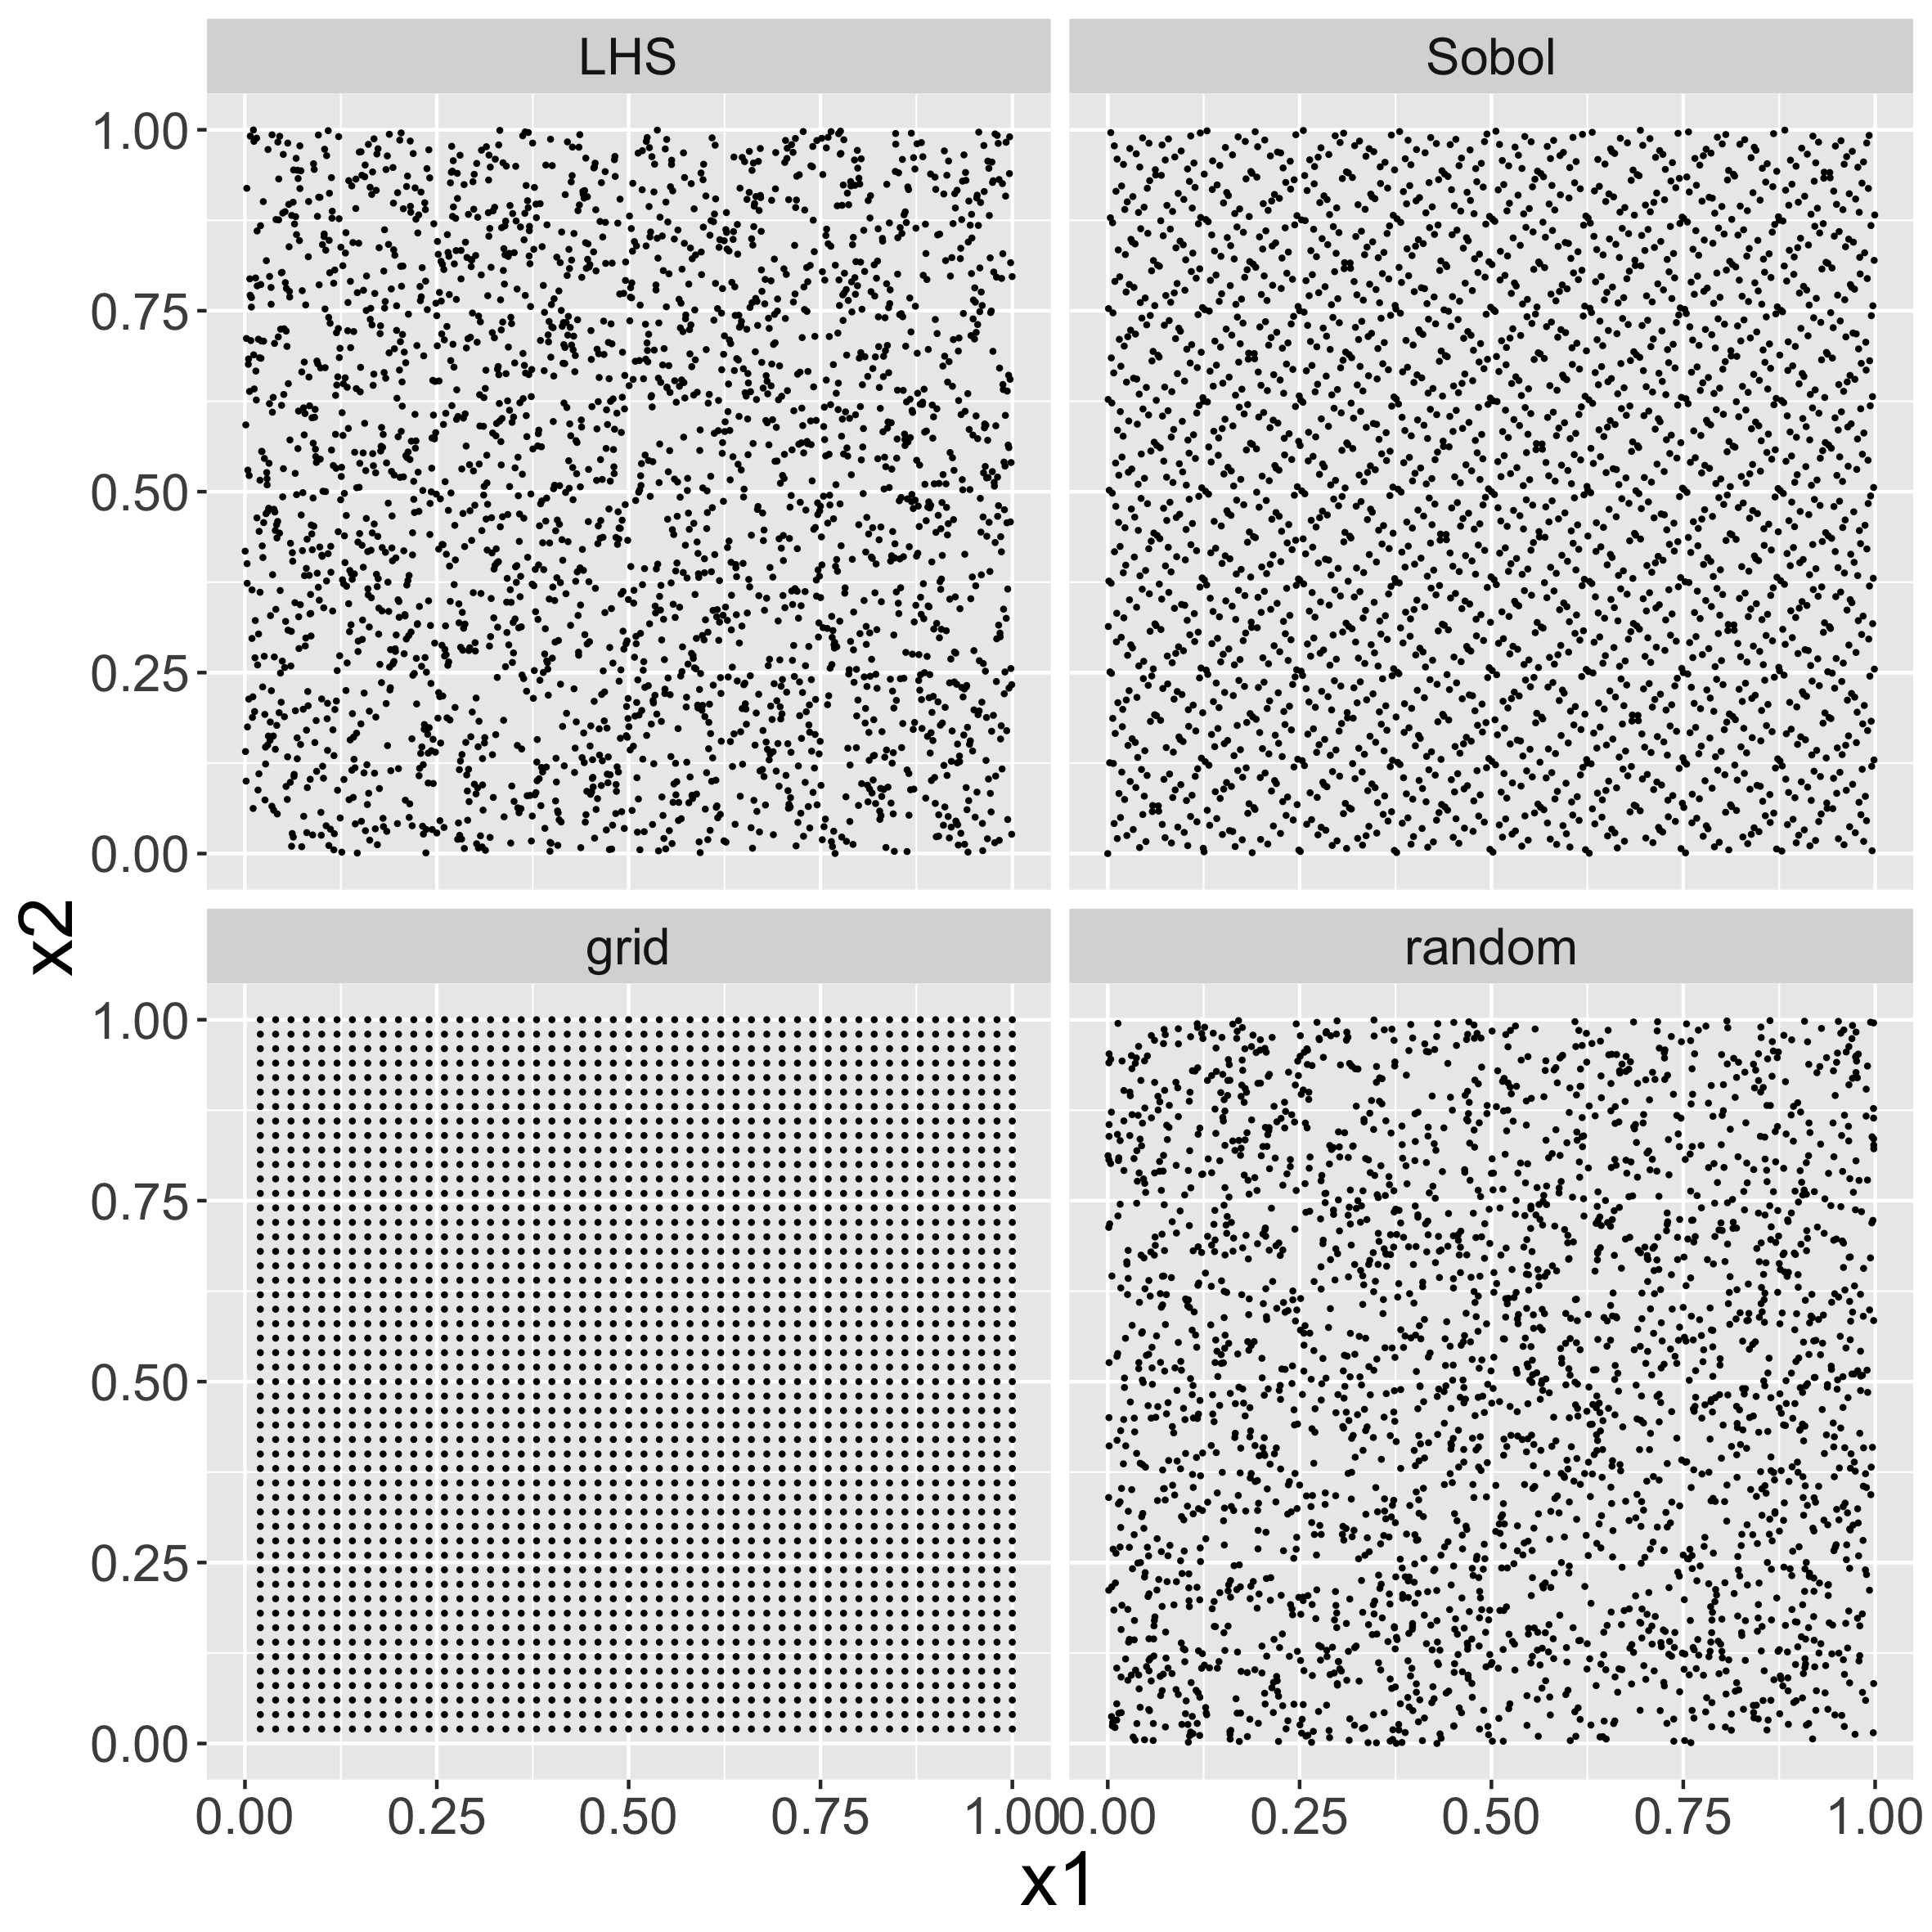
\includegraphics[height=0.8\textheight]{figures/sobol.png}

}

\sframe{Comparison of samplings}{

\textit{Estimated discrepancies for repetitions of samplings as a function of sample size}

\centering

\medskip

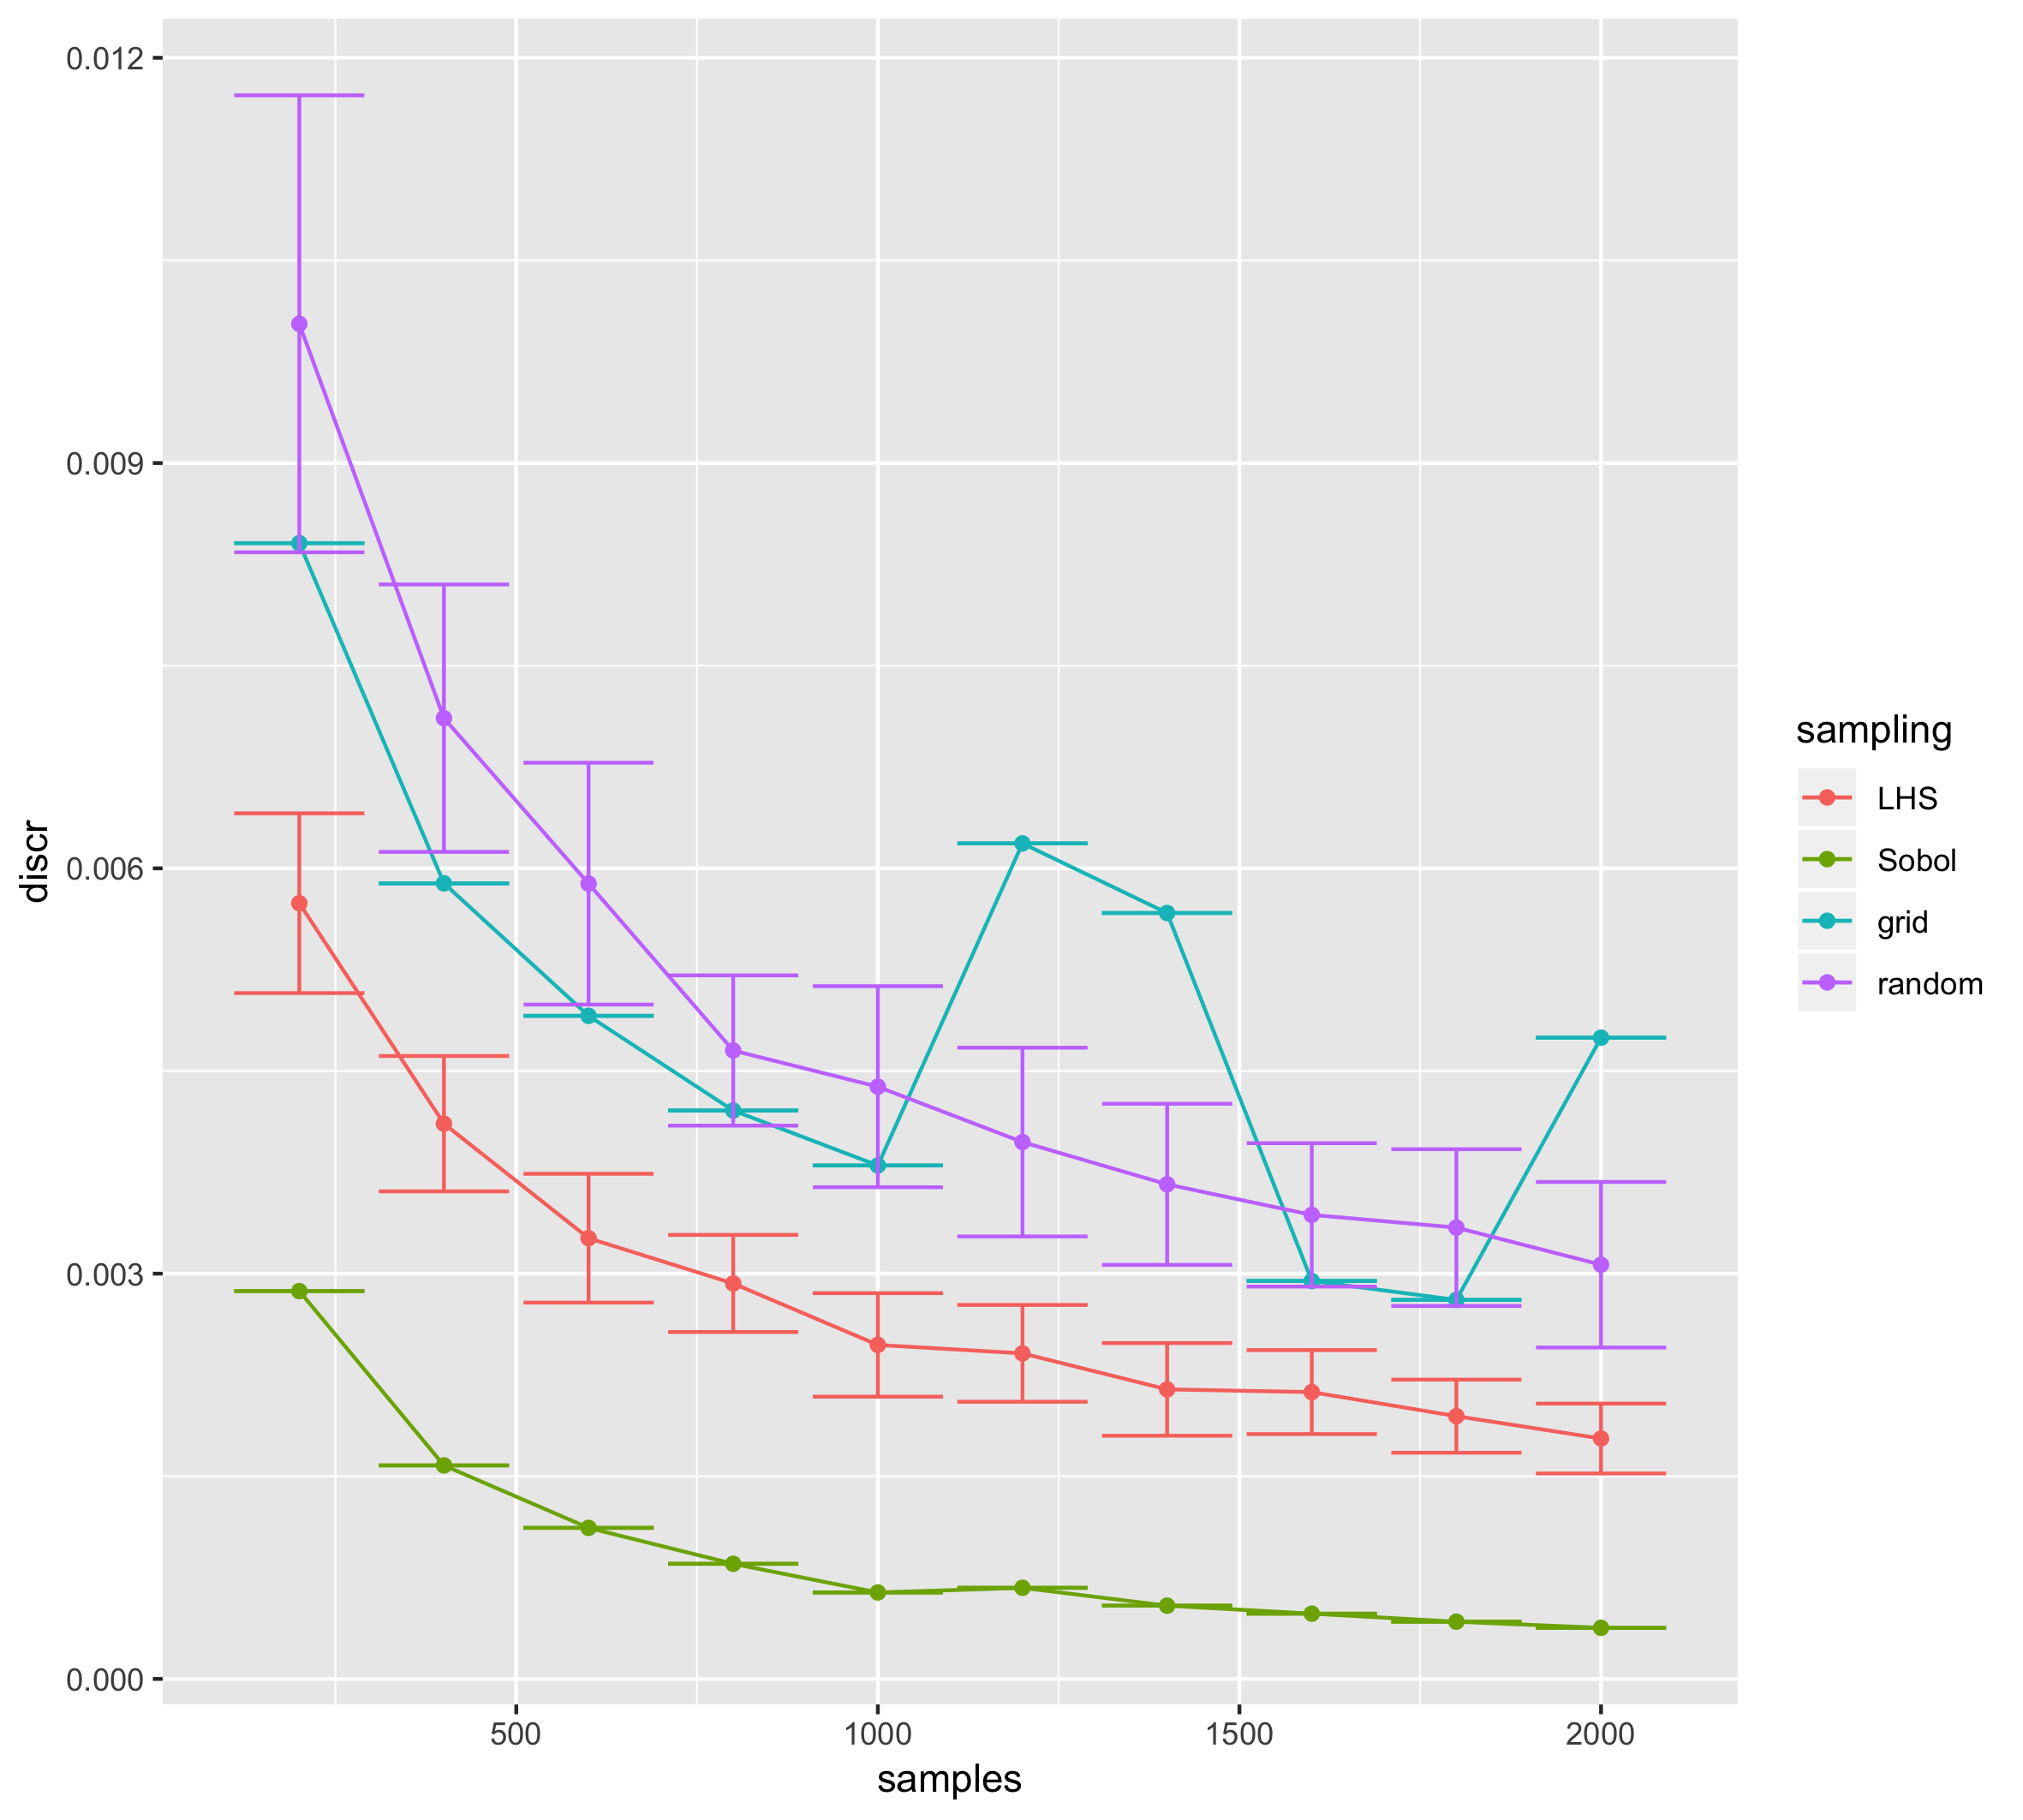
\includegraphics[height=0.8\textheight]{figures/discrepancies.png}

}



\sframe{Syntax of high-dimensional samplings}{

\textbf{LHS Sampling}
  
\texttt{
sampling = LHS(\\
\hspace{1cm}100,\\
\hspace{1cm}x1 in (0.0,1.0),\\
\hspace{1cm}x2 in (0.0,1.0)\\
)
}

\bigskip

\textbf{Sobol sampling}

\texttt{
sampling = SobolSampling(\\
\hspace{1cm} 100,\\
\hspace{1cm}x1 in (0.0,1.0),\\
\hspace{1cm}x2 in (0.0,1.0)\\
)
}

\bigskip

$\rightarrow$ \textbf{Practice: } test these samplings in \texttt{directsampling.oms}



}

%\sframe{Result examples for the Zombie model}{
%%  plots direct sampling -> above
%}


\sframe{Summary}{

\textbf{Summary of samplings characteristics}

\bigskip
\bigskip

\begin{columns}
	\begin{column}{0.35\linewidth}
	
	\bigskip
	\bigskip
	
	One factor at a time
	
	\medskip
	
	Complete plan
	
	\medskip
	
	LHS/Sobol
		
	\end{column}
	\begin{column}{0.2\linewidth}
		
		\textbf{Coverage}
		
		\bigskip
		
		{\textcolor{red}
		\xmark
		}
		
		\medskip
		
		{\textcolor{green}
		\cmark
		}
		
		\medskip
		
		{\textcolor{green}
		\cmark
		}
			
	\end{column}
	
	\begin{column}{0.25\linewidth}
		
		\textbf{Interpretability}
		
		\bigskip
		
		{\textcolor{green}
		\cmark
		}
		
		\medskip
		
		{\textcolor{green}
		\cmark
		}
		
		\medskip
		
		{\textcolor{red}
		\xmark
		}	
	\end{column}
	
	\begin{column}{0.2\linewidth}
		
		\textbf{Budget}
		
		\bigskip
		
		{\textcolor{green}
		\cmark
		}
		
		\medskip
		
		{\textcolor{red}
		\xmark
		}
		
		\medskip
		
		{\textcolor{green}
		\cmark
		}	
	\end{column}

	
	
	
\end{columns}


}





\section{Sensitivity analysis}


\sframe{Sensitivity analysis}{

\textbf{Aim of sensitivity analysis methods} \textit{How to summarize model sensitivity and isolate principal factors ?}

\bigskip


 \begin{itemize}
 	\item Most methods are \textit{global}, i.e. provide an aggregate of factor effect on the full parameter space
 	\item Advanced methods, still useful for preliminary experiments e.g. to discard factors from further experiments
 	\item Examples: Morris and Saltelli methods
 \end{itemize}



}



\sframe{Morris method}{

\justify

\textbf{Idea: } \textit{Sample trajectories in the parameter space in a One-At-a-Time manner. Screening method isolating \textbf{elementary effects}}

\bigskip

\begin{itemize}
  \item isolate local effects of factors
  \item more efficient than point sampling to get individual effects
  \item useful as a first experiment to understand the relative influence of factors
\end{itemize}

\bigskip

Introduced by \cite{morris1991factorial}, improved by \cite{saltelli2004sensitivity},\\
 \cite{campolongo2011screening} propose to extend the method with Sobol sequences



}

\sframe{Morris method}{

\justify

Let $\delta$ be step for parameter variation (all assumed normalized in $[0;1]$), the \textit{elementary effect} for parameter $i$ on output $Y$ at point $\vec{x}$ is given by 

\[
\varepsilon_i (\vec{x}) = \frac{Y(\vec{x}+\delta\cdot \vec{e}_i) - Y(\vec{x})}{\delta}
\]

With $N$ parameter trajectories randomly sampled (each trajectory varying all parameters), the sensitivity index is given by
\[
\mu_i = \frac{\sum_{k=1}^N \varepsilon_i (\vec{x}_k)}{N}
\]
and complementary indices by

\[
\sigma_i = \frac{\sum_{k=1}^N \left(\varepsilon_i (\vec{x}_k) - \mu_i\right)^2}{N}
\]

\[
\mu^{\ast}_i = \frac{\sum_{k=1}^N \left|\varepsilon_i (\vec{x}_k)\right|}{N}
\]

}


\sframe{Morris}{

\textit{In OpenMOLE, Morris is a method in itself (and not a sampling)}

\bigskip

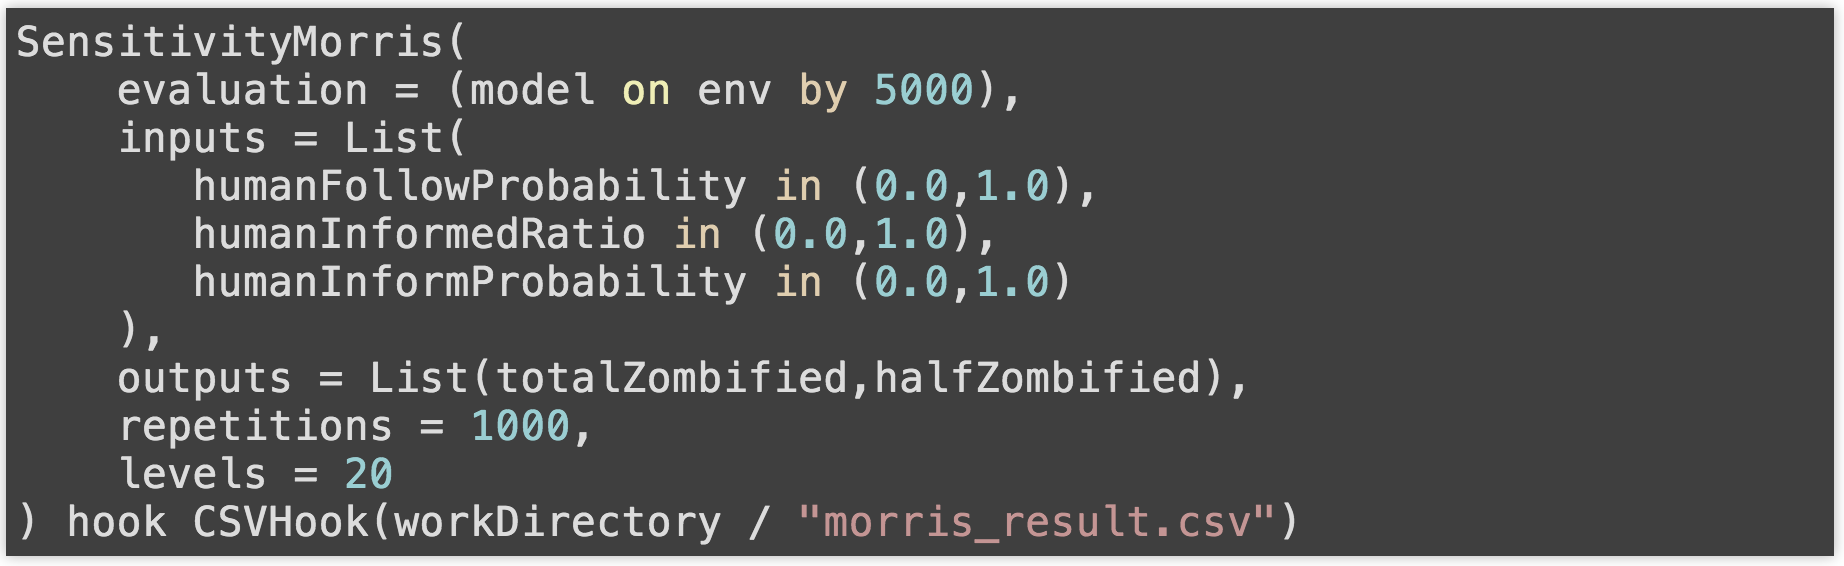
\includegraphics[width=\textwidth]{figures/morris_code.png}

\bigskip

$\rightarrow$ \textbf{Practice: } explore the script \texttt{morris.oms}, comment the results obtained with a large-scale experiment \texttt{morrisresults}

}



\sframe{Saltelli method}{

\textit{Method based on the estimation of conditional relative variances}

\cite{saltelli2010variance}

\medskip

\textbf{First order index}

\[
S_i = \frac{Var \left[ E_{\mathbf{X}_{\sim i}} (Y | X_i ) \right]}{Var(Y)}
\]

is the expected relative variance reduction if $X_i$ would be fixed

\medskip

\textbf{Total effect index}
\[
ST_i = \frac{E_{\mathbf{X}_{\sim i}}\left[Var(Y | \mathbf{X}_{\sim i}) \right]}{Var(Y)}
\]

is the expected relative variance if all factors but $X_i$ are fixed (includes interaction effects)

%for factor $i$ gives the variance of indicator $Y$ conditionally to all other factors being fixed, relative to indicator variance.



}

\sframe{Saltelli}{

\justify

\textit{In OpenMOLE, Saltelli is also a method}

\bigskip


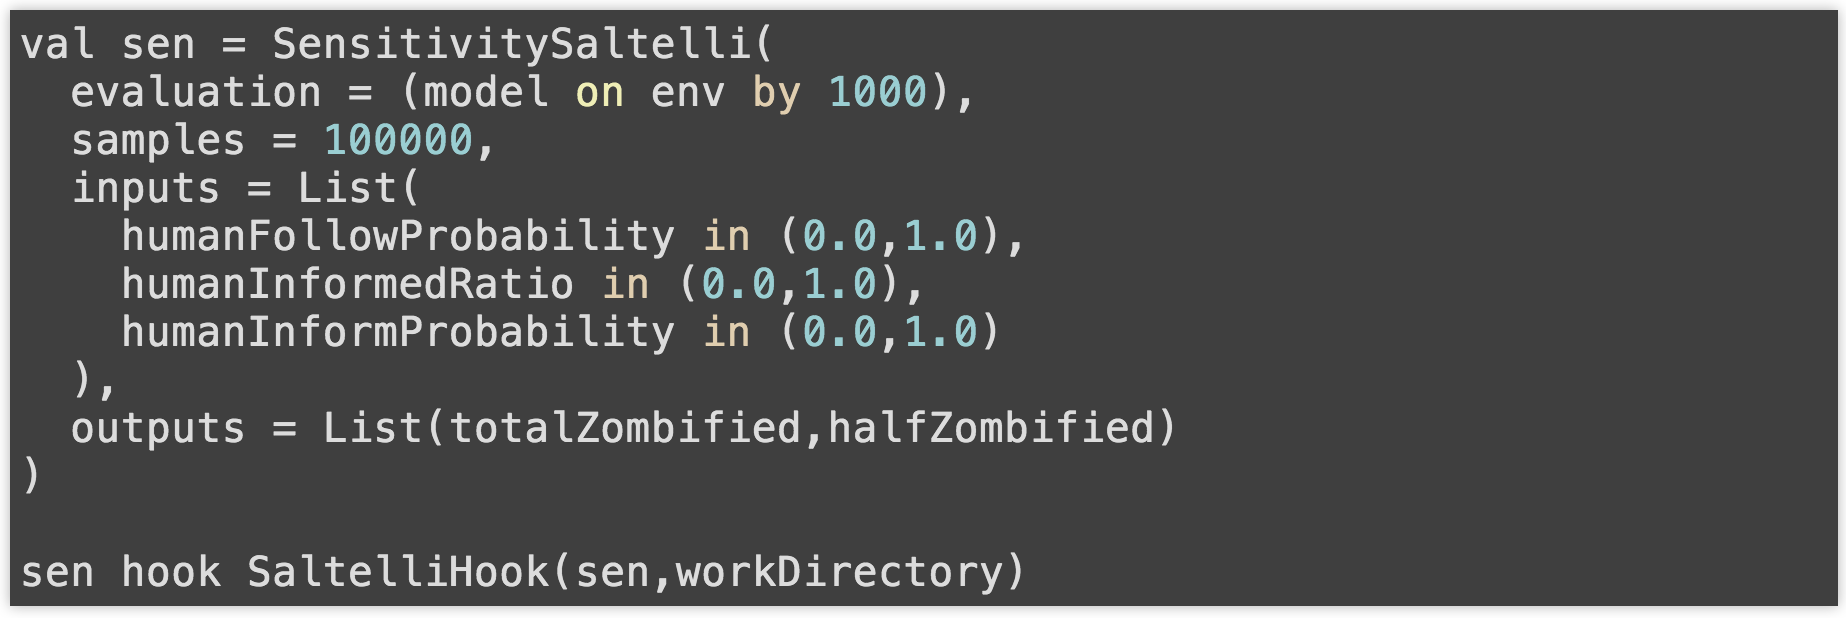
\includegraphics[width=\textwidth]{figures/saltellicode.png}


}



\sframe{Summary}{

\textbf{Summary of sensitivity methods}

\bigskip
\bigskip

\begin{columns}
	\begin{column}{0.35\linewidth}
	
	\bigskip
	\bigskip
	
	Morris
	
	\medskip
	
	Saltelli
	

		
	\end{column}
	\begin{column}{0.2\linewidth}
		
		\textbf{Coverage}
		
		\bigskip
		
		{\textcolor{red}
		\xmark
		}
		
		\medskip
		
		{\textcolor{green}
		\cmark
		}
		
	
			
	\end{column}
	
	\begin{column}{0.25\linewidth}
		
		\textbf{Interpretability}
		
		\bigskip
		
		{\textcolor{green}
		\cmark
		}
		
		\medskip
		
		{\textcolor{green}
		\cmark
		}
			
	\end{column}
	
	\begin{column}{0.2\linewidth}
		
		\textbf{Budget}
		
		\bigskip
		
		{\textcolor{green}
		\cmark
		}
		
		\medskip
		
		{\textcolor{red}
		\xmark
		}
			
	\end{column}

	
	
	
\end{columns}


}





\sframe{Conclusion}{

\textbf{Take-home messages: }

\medskip

\begin{itemize}
	\item Direct sampling can be useful as preliminary experiments, but also experiments in themselves
	\item Sensitivity analysis methods are useful for a global knowledge on influence of factors
	\item Find a good balance interpretability/computational budget/information extracted
	\item The experiments you choose depend on your questions but also on your discipline
\end{itemize}

}











%\backupbegin

%\appendix


%\sframe{Results of grid exploration}{

%\textit{Cooperation model}

%}




%%%%%%%%%%%%%%%%%%%%%
\begin{frame}[allowframebreaks]
\frametitle{References}
\bibliographystyle{apalike}
\bibliography{biblio}
\end{frame}
%%%%%%%%%%%%%%%%%%%%%%%%%%%%


%\backupend





\end{document}


